%
%%%%%%%%%%%%%%%%%%%%%%% file typeinst.tex %%%%%%%%%%%%%%%%%%%%%%%%%
%
% This is the LaTeX source for the instructions to authors using
% the LaTeX document class 'llncs.cls' for contributions to
% the Lecture Notes in Computer Sciences series.
% http://www.springer.com/lncs       Springer Heidelberg 2006/05/04
%
% It may be used as a temlpate for your own input - copy it
% to a new file with a new nam eand use it as the basis
% for your article.
%
% NB: the document class 'llncs' has its own and detailed documentation, see
% ftp://ftp.springer.de/data/pubftp/pub/tex/latex/llncs/latex2e/llncsdoc.pdf
%
%%%%%%%%%%%%%%%%%%%%%%%%%%%%%%%%%%%%%%%%%%%%%%%%%%%%%%%%%%%%%%%%%%%


\documentclass[runningheads,a4paper]{llncs}

\usepackage{amssymb}
\setcounter{tocdepth}{3}
\usepackage{graphicx}
\usepackage{amsmath}
\usepackage{booktabs}
%\usepackage{times}
\usepackage{perpage}
\usepackage{hyperref}
\MakePerPage{footnote}
\usepackage{multirow}
\usepackage{epstopdf} %converting to PDF
\usepackage{tikz}
\usetikzlibrary{arrows,patterns,automata,backgrounds,decorations,fit,petri,positioning,petri,shapes,calc}
\usepackage[caption=false]{subfig}
\usepackage{url}

\urldef{\mailsa}\path|{andriiro,f.m.maggi,marlon.dumas}@ut.ee, kerwin.jorbina@gmail.com|
\urldef{\mailsb}\path|dfmchiara@fbk.eu|
\urldef{\mailsc}\path|{ilya.verenich,m.larosa,simon.raboczi}@qut.edu.au|
\newcommand{\keywords}[1]{\par\addvspace\baselineskip
\noindent\keywordname\enspace\ignorespaces#1}

\begin{document}

\mainmatter  % start of an individual contribution

% first the title is needed
\title{Nirdizati: A Web-based Tool for Predictive Process Monitoring}

% a short form should be given in case it is too long for the running head
\titlerunning{Predictive Business Process Monitoring with LSTM Neural Networks}

% the name(s) of the author(s) follow(s) next
%
% NB: Chinese authors should write their first names(s) in front of
% their surnames. This ensures that the names appear correctly in
% the running heads and the author index.
%
\author{Andrii Rozumnyi\inst{1} \and Chiara Di Francescomarino\inst{2} \and Fabrizio Maria Maggi\inst{1} \and \\Ilya Verenich\inst{3,1} \and Kerwin Jorbina\inst{1} \and Marcello La Rosa\inst{3} \and \\ Marlon Dumas\inst{1} \and Simon Raboczi\inst{3}\thanks{Author names are in alphabetical order}}

\institute{University of Tartu, Estonia\\
\mailsa
\and FBK IRST, Trento, Italy\\
\mailsb
\and Queensland University of Technology, Australia\\
\mailsc
}

%
% NB: a more complex sample for affiliations and the mapping to the
% corresponding authors can be found in the file "llncs.dem"
% (search for the string "\mainmatter" where a contribution starts).
% "llncs.dem" accompanies the document class "llncs.cls".
%

\toctitle{Predictive Process Monitoring Using LSTM}
\tocauthor{Authors' Instructions}
\maketitle


\begin{abstract}
In this paper, we present Nirdizati, an open-source tool for predictive monitoring of business processes.
The tool can be used to predict the outcome, the next events, or the remaining time of each case of a process.
For example, in an lead-to-order process, Nirdizati can predict which customer leads will convert to purchase orders and when.
In a claims handling process, Nirdizati can predict if a claim decision will be made on time or late.
Based on these predictions, process workers and operational managers can act proactively to resolve or mitigate potential process performance violations.
The target audience of this demonstration includes process mining researchers as well as practitioners interested in exploring the potential of process monitoring.
\keywords{Process Mining, Predictive Process Monitoring, Machine Learning}
\end{abstract}


\section{Introduction} \label{sec:intro}
Nirdizati consists of two components: Nirdizati Training and Nirdizati Runtime (Figure~\ref{fig:nirdizati-overall}). Nirdizati Training takes as input a business process event log and produces a prediction model. This model can then be deployed in Nirdizati Runtime. Once a model is deployed, Nirdizati Runtime listens to a stream of events related to a business process, and produces a stream of predictions. These predictions are then visualized in a continuously updated Web dashboard.

%\vspace{-\baselineskip}
\begin{figure}[t]%[H]
	\centering
	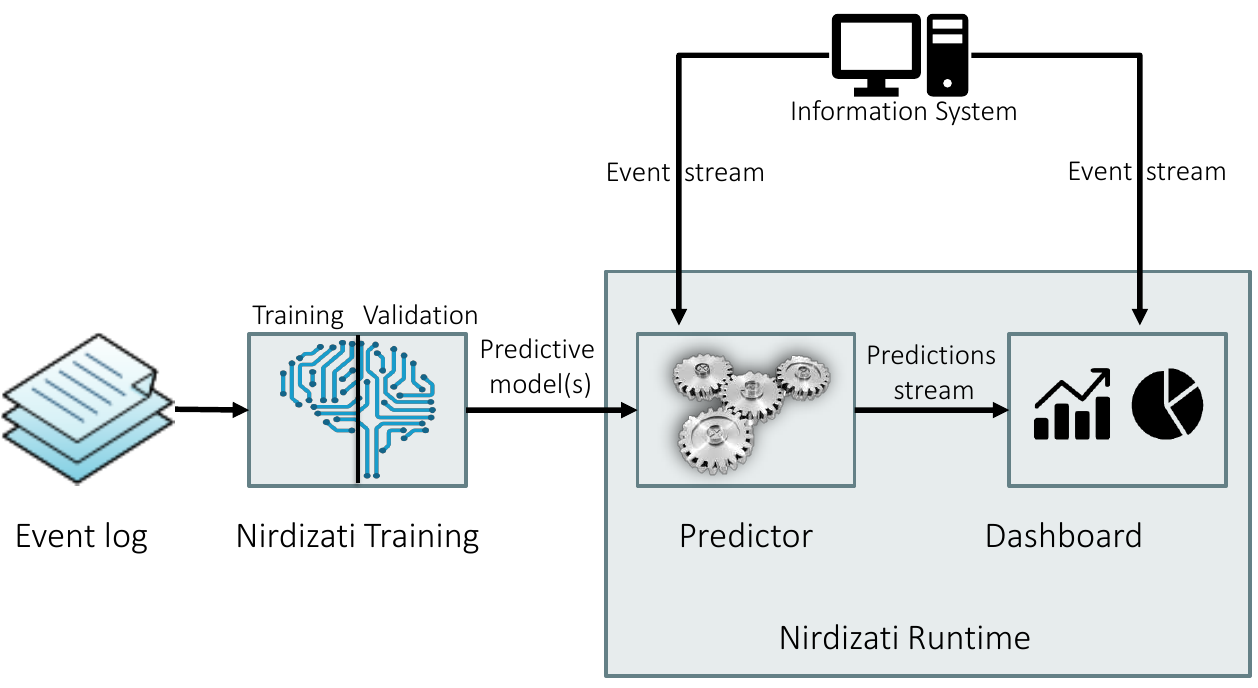
\includegraphics[width=0.7\textwidth]{img/nirdizati-overall}
	\caption{A high-level overview of Nirdizati.}
	\label{fig:nirdizati-overall}
\end{figure}
%\vspace{-\baselineskip}


\section{Nirdizati Training} \label{sec:training}
First, we have the Front-end application which acts as the interface for the user to
select settings used for prediction and to analyze the prediction results. The second
module is the Log Manager which is responsible for managing the logs. Uploading
and retrieving the logs are the basic operations of this module. The third module is
the Encoder which retrieves the log from the storage, parses it and prepares the log for
the training phase in the Predictive Module. In this part, we retrieve the encoded data,
split it into training and test set for evaluation, and build the predictive model from the
training data. Finally, using the test data, we test it against the model created to get its
accuracy. The aggregation of the results are done in the Evaluation Module which is
tasked to calculate the error of the prediction model created.


%\vspace{-\baselineskip}
\begin{figure}[t]%[H]
	\centering
	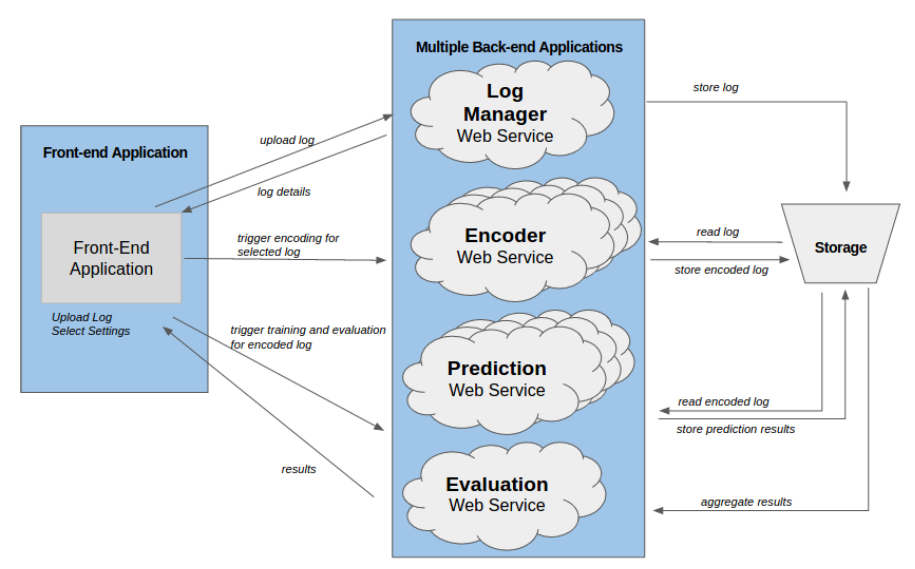
\includegraphics[width=0.7\textwidth]{img/nirdizati-training}
	\caption{A high-level overview of Nirdizati Training.}
	\label{fig:nirdizati-training}
\end{figure}
%\vspace{-\baselineskip}

\section{Nirdizati Runtime} \label{sec:runtime}
Figure~\ref{fig:dfd_0} illustrates the flow of data through the proposed system. A workflow management system (WFMS) continuously registers tasks performed in the organization.
This serves as an input to our system, in the form of a stream of events.
Next, the produced stream is consumed by a web server which is responsible for storing data and further information processing. 
Web server, in turn, communicates with a predictive engine which applies pre-trained models for a business process and returns all the results of calculations.
After web server receives the outputs from each predictive model, it writes them to a database and updates corresponding clients.
From the user's side, the results are visualized via a dashboard-based interface which is capable of sending queries requesting various visualization options.


\begin{figure}
	\centering
	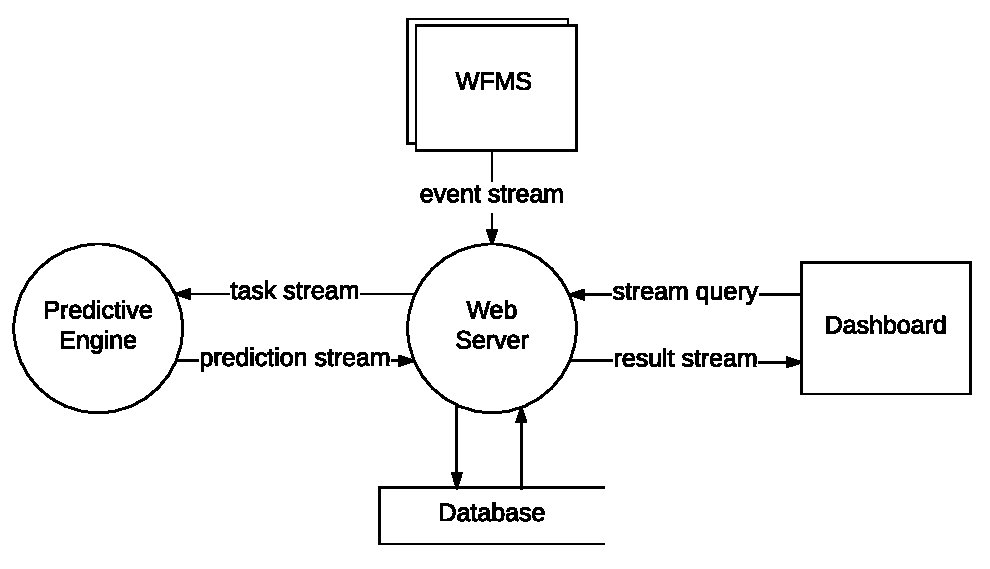
\includegraphics[width=0.7\textwidth]{img/dfd_0}
	\caption{High-level data flow diagram in a Yourdon-Coad notation}
	\label{fig:dfd_0}
\end{figure}

Based on this data flow diagram, we devise the main parts and high-level components of the system (Figure~\ref{fig:nirdizati-runtime}): 

\begin{itemize}
	\setlength{\itemsep}{1pt}
	\setlength{\parskip}{0pt}
	\setlength{\parsep}{0pt}
	\item streaming platform
	\item web server with load balancer and internal components
	\item predictive engine
	\item client-side user interfaces
\end{itemize}

\begin{figure}
	\centering
	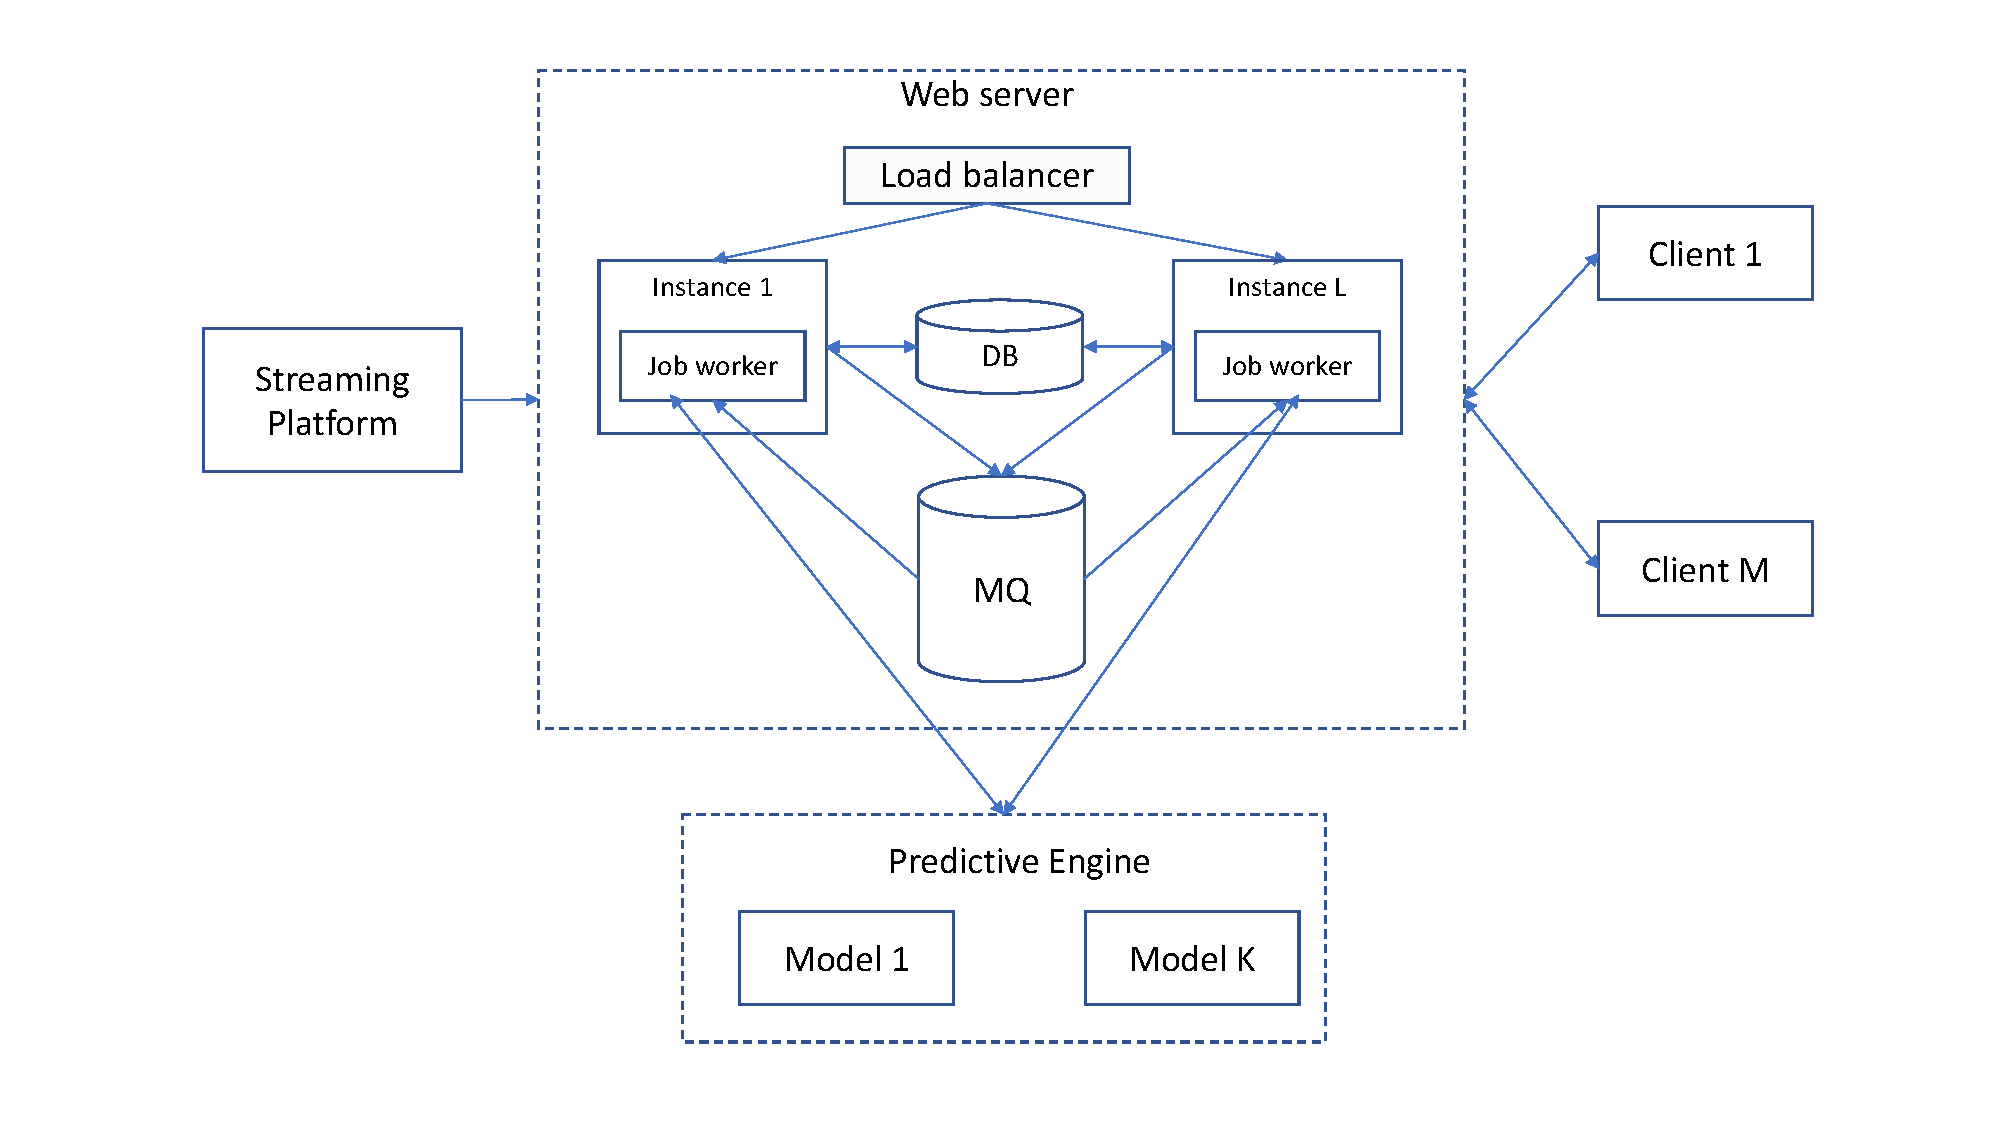
\includegraphics[width=1\textwidth]{img/nirdizati-runtime}
	\caption{Proposed system design architecture}
	\label{fig:nirdizati-runtime}
	%	\vspace{-5\baselineskip}
\end{figure}

Process workers and operational managers – typical users of such system – can set the process performance targets and subscribe to a stream of warnings and alerts generated whenever these targets are predicted to be violated. Thus, process workers will be capable of making more informed, data-driven decisions to get a better control of the process execution. This is especially beneficial for processes where process workers have more leeway to make corrective actions, for example, in a lead management process.

\section{Conclusion} \label{sec:conclusion}
The developed solution, named \emph{Nirdizati}, is a configurable full-stack web application that supports users in selecting the preferred prediction method from the list of implemented methods and enables the continuous prediction of various performance indicators at runtime.
The results of the predictions, as well as the real-time summary statistics about the process execution, are presented in a dashboard that offers multiple visualization options.

The source code has been released as open source software under the Lesser GNU Public License (L-GPL) at \url{http://github.com/nirdizati}. The developed engine has been deployed on the server belonging to the Institute of Computer Science and can be accessed at \url{http://nirdizati.com}.
\bibliographystyle{splncs03}
\bibliography{paper}

\end{document}
